\documentclass[a4paper, 12pt]{article}
\usepackage[utf8]{inputenc}
\usepackage{url}
\usepackage{amsmath, amssymb, amsfonts}
\usepackage{graphicx}

\begin{document}
\begin{center}
{\LARGE \bf Praktikum Wissenschaftliches Rechnen \\ \vspace{0.2cm} (CFD, Final Project)}\\
\vspace{0.6cm}
{\small Group 9: Breznik, E., Cheng, Z., Ni, W., Schmidbartl, N.}
\end{center}
\normalfont
\section{The Topic}\label{sec:topic}
For the final project, our group chose to extend the Navier Stokes code to be used in 3D for arbitrary geometries, with the ability of handling
the Free Surface flow scenarios.
We put a lot of attention to designing a code that will work in 3D for as many different scenarios as possible. That is why we did not code a
special set of boundaries for just a few more known and frequently simulated situations, but rather made them completely dependent on the input
geometry file.

%TODO:comment on not doing free surface
\subsection{Running the program}
Program is called in the same way as its 2D version;
\begin{center} 
\begin{verbatim}
./sim parameter_file
\end{verbatim}
\end{center}
with parameter\_file denoting the usual (only slightly extended) parameter file, where (under variable name $problemGeometry$) also the geometry file is 
given - see next section for more information on input. 

\subsection{Input}\label{sec:input}
The parameter file that was used as input in our previous worksheets remained, with just slight changes due to the additional dimension.
Only notable difference is, that we now take as an input also a scalar $velIN$, and a vector $velMW$. First one represent the velocity at the
inflow boundaries, and the second one the wall velocity for the moving wall boundaries. %TODO: when describin these b.c. say more about the velocity, what it represents

To make our code able to handle truly arbitrary scenarios, we designed so that it allows for any sort of implemented boundary conditions to be employed in any
domain cell - so even the obstacles inside the domain can have arbitrary boundaries, as opposed to only allowing that on the domain walls (as in worksheet 3).
The standard boundary conditions, that we implemented, are
\begin{itemize}
\item no slip,
\item free slip,
\item inflow,
\item outflow,
\item moving wall.
\end{itemize}
To specify, where which of them is applied, we used special numbering of cells when generating our input pgm files, which can be seen from table
1, so our geometries are represented by a grayscale image with 7 levels of brightness.
\begin{table}[hb!]
\centering
\label{tab1}
\begin{tabular}{|l|c|}
\hline
{\bf Cell type} & {\bf Number code}\\
\hline
water & 0 \\
air & 1 \\
no-slip & 2 \\
free-slip & 3 \\
inflow & 4 \\
outflow & 5 \\
moving wall & 6 \\
\hline
\end{tabular}
\caption{Number representations of different possible cell types.}
\end{table}
Since we are working in three dimensions, this image consists of a sequence of 2D ($xy$ plane) images. The orientation of coordinate system and an
example picture for a small lid driven cavity case can be seen on figure 1. One geometry picture set thus needs to contain
$(imax+2)\times(jmax+2)\times(kmax+2)$ numbers in $(jmax+2)\times(kmax+2)$ rows, and is typically very big.
\begin{figure}[ht!]
\centering
\label{fig1}
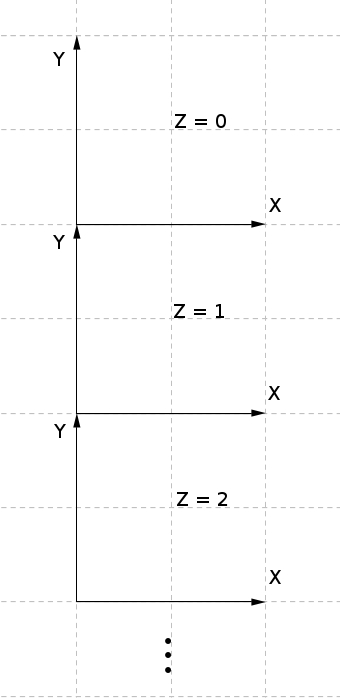
\includegraphics[height=6.2cm]{coord.jpg}
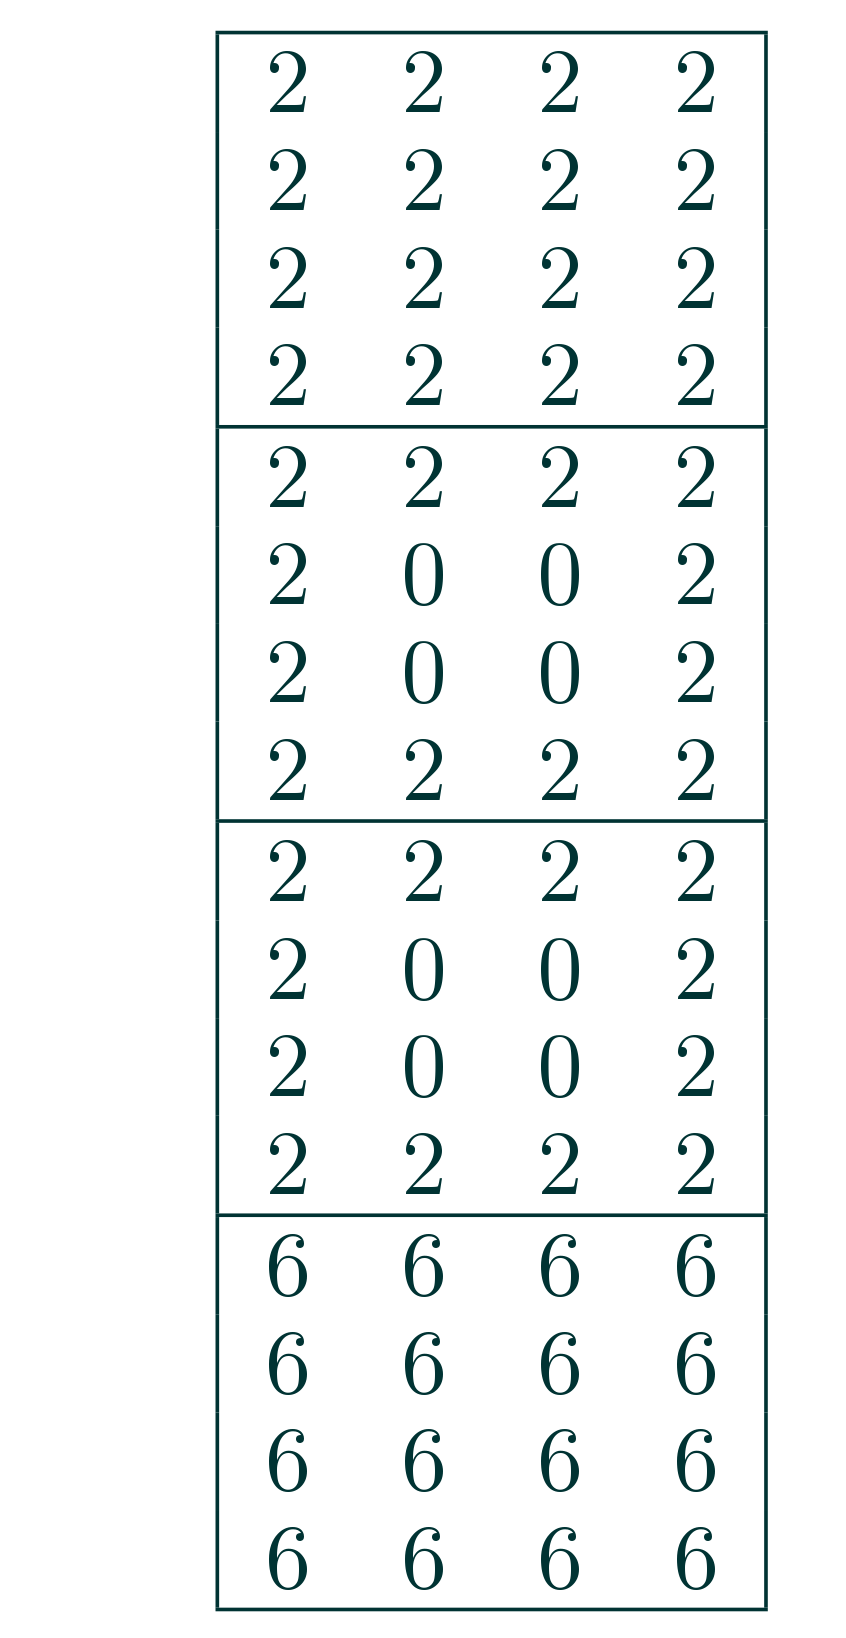
\includegraphics[height=6.2cm]{cavity.png}

\includegraphics[height=6cm]{cavity20202.jpg}
\caption{The structure of our input pgm files and a lid driven cavity example case.}
\end{figure}


\section{Implementation}\label{sec:implement}
\subsection{Boundary conditions}\label{sec:boundary_vel}
As mentioned before, we have implemented 5 different boundary conditions for the 6 boundaries of our 3D domain, as well as for internal boundaries.
\subsubsection{No-Slip boundary condition}\label{sec:no-slip}
For no-slip conditions, the fluid vanishes at the boundary. As a consequence, both the velocity components are zero. 
%Using staggered grid, the discrete velocity components normal to and parallel to the boundary lie directly at the boundary, whilst the one parallel to the boundary is the average of the boundary cell's and its neighbouring fluid cell's velocity components.

%Therefore, for the \texttt{B\_O} case, we set the following boundary conditions:
%\begin{equation}
%\begin{array}{lll}
%u_{i,j,k} = 0, & v_{i,j-1,k} = -v_{i+1,j-1,k}, & v_{i,j,k} = -v_{i+1,j,k}, \\
%w_{i,j,k-1} = -w_{i+1,j,k-1}, & w_{i,j,k} = -w_{i+1,j,k},& \\
%\end{array}
%\end{equation}
%and we analogously set the boundary conditions for the following 5 cases: \texttt{B\_W}, \texttt{B\_N}, \texttt{B\_S}, \texttt{B\_U} and \texttt{B\_D}.
%
%For the \texttt{B\_NO} case, we set the following boundary conditions:
%\begin{equation}
%\begin{array}{ll}
%u_{i,j,k} = 0, & u_{i-1,j,k} = -u_{i-1,j+1,k}, \\
%v_{i,j,k} = 0, & v_{i,j-1,k} = -v_{i+1,j-1,k}, \\
%w_{i,j,k} = -\frac{1}{2}(w_{i+1,j,k}+w_{i,j+1,k}), &
%w_{i,j,k-1} = -\frac{1}{2}(w_{i+1,j,k-1}+w_{i,j+1,k-1}), \\
%\end{array}
%\end{equation}
%and we analogously set the boundary conditions for the following 11 cases: \texttt{B\_NW}, \texttt{B\_NU}, \texttt{B\_ND}, \texttt{B\_SO}, \texttt{B\_SW}, \texttt{B\_SU}, \texttt{B\_SD}, \texttt{B\_OU}, \texttt{B\_WU}, \texttt{B\_OD} and \texttt{B\_WD}.

For the \texttt{B\_NOU} case, we set the following boundary conditions:
\begin{equation}
\begin{array}{ll}
u_{i,j,k} = 0, & u_{i-1,j,k} = -\frac{1}{2}(u_{i-1,j+1,k}+u_{i-1,j,k+1}), \\
v_{i,j,k} = 0, & v_{i,j-1,k} = -\frac{1}{2}(v_{i+1,j-1,k}+v_{i+1,j-1,k+1}), \\
w_{i,j,k} = 0, & w_{i,j,k-1} = -\frac{1}{2}(w_{i+1,j,k-1}+w_{i,j+1,k-1}), \\
\end{array}
\end{equation}
and we analogously set the boundary conditions for the following 7 cases: \texttt{B\_NWU}, \texttt{B\_NOD}, \texttt{B\_NWD}, \texttt{B\_SOU}, \texttt{B\_SWU}, \texttt{B\_SOD}, and \texttt{B\_SWD}.

Boundary conditions of the cells that only have one or two fluid neighbours are analogous to their 2D counterparts, and are omitted here for the sake of brevity;
same applies for the discussion in  \ref{sec:free-slip}, \ref{sec:outflow}, and \ref{sec:boundary_pressure}.

%\texttt{B\_O}, \texttt{B\_W}, \texttt{B\_N}, \texttt{B\_S}, \texttt{B\_U}, \texttt{B\_D}; \texttt{B\_NO} \texttt{B\_NW}, \texttt{B\_NU}, \texttt{B\_ND}, \texttt{B\_SO}, \texttt{B\_SW}, \texttt{B\_SU}, \texttt{B\_SD}, \texttt{B\_OU}, \texttt{B\_WU}, \texttt{B\_OD} and \texttt{B\_WD}. 

\subsubsection{Free-Slip boundary condition}\label{sec:free-slip}
For free-slip conditions, the fluid flows freely parallel to the boundary, but does not cross the boundary. As a consequence, the velocity component normal to the boundary is zero, as well as the normal derivative of the velocity component parallel to the wall. 
%Using staggered grid, the discrete velocity components normal to the boundary lie directly at the boundary, whilst the one parallel to the boundary is the average of the boundary cell's and its neighbouring fluid cell's velocity components.
%
%Therefore, for the \texttt{B\_O} case, we set the following boundary conditions:
%\begin{equation}
%\begin{array}{lll}
%u_{i,j,k} = 0, & v_{i,j-1,k} = v_{i+1,j-1,k}, & v_{i,j,k} = v_{i+1,j,k}, \\
%w_{i,j,k-1} = w_{i+1,j,k-1}, & w_{i,j,k} = w_{i+1,j,k},& \\
%\end{array}
%\end{equation}
%and we analogously set the boundary conditions for the following 5 cases: \texttt{B\_W}, \texttt{B\_N}, \texttt{B\_S}, \texttt{B\_U} and \texttt{B\_D}.
%
%For the \texttt{B\_NO} case, we set the following boundary conditions:
%\begin{equation}
%\begin{array}{ll}
%u_{i,j,k} = 0, & u_{i-1,j,k} = u_{i-1,j+1,k}, \\
%v_{i,j,k} = 0, & v_{i,j-1,k} = v_{i+1,j-1,k}, \\
%w_{i,j,k} = \frac{1}{2}(w_{i+1,j,k}+w_{i,j+1,k}), &
%w_{i,j,k-1} = \frac{1}{2}(w_{i+1,j,k-1}+w_{i,j+1,k-1}), \\
%\end{array}
%\end{equation}
%and we analogously set the boundary conditions for the following 11 cases: \texttt{B\_NW}, \texttt{B\_NU}, \texttt{B\_ND}, \texttt{B\_SO}, \texttt{B\_SW}, \texttt{B\_SU}, \texttt{B\_SD}, \texttt{B\_OU}, \texttt{B\_WU}, \texttt{B\_OD} and \texttt{B\_WD}.

For the \texttt{B\_NOU} case, we set the following boundary conditions:
\begin{equation}
\begin{array}{ll}
u_{i,j,k} = 0, & u_{i-1,j,k} = \frac{1}{2}(u_{i-1,j+1,k}+u_{i-1,j,k+1}), \\
v_{i,j,k} = 0, & v_{i,j-1,k} = \frac{1}{2}(v_{i+1,j-1,k}+v_{i+1,j-1,k+1}), \\
w_{i,j,k} = 0, & w_{i,j,k-1} = \frac{1}{2}(w_{i+1,j,k-1}+w_{i,j+1,k-1}), \\
\end{array}
\end{equation}
and we analogously set the boundary conditions for the following 7 cases: \texttt{B\_NWU}, \texttt{B\_NOD}, \texttt{B\_NWD}, \texttt{B\_SOU}, \texttt{B\_SWU}, \texttt{B\_SOD}, and \texttt{B\_SWD}.

\subsubsection{Outflow boundary condition}\label{sec:outflow}
For outflow conditions, the normal derivatives of both the velocity components are zero. 
%Using staggered grid, the discrete velocity component normal to the boundary lie directly at the boundary, whilst the one parallel to the boundary is the average of the boundary cell's and its neighbouring fluid cell's velocity components.
%
%Therefore, for the \texttt{B\_O} case, we set the following boundary conditions:
%\begin{equation}
%\begin{array}{lll}
%u_{i,j,k} = u_{i+1,j,k}, & v_{i,j-1,k} = v_{i+1,j-1,k}, & v_{i,j,k} = v_{i+1,j,k}, \\
%w_{i,j,k-1} = w_{i+1,j,k-1}, & w_{i,j,k} = w_{i+1,j,k},& \\
%\end{array}
%\end{equation}
%and we analogously set the boundary conditions for the following 5 cases: \texttt{B\_W}, \texttt{B\_N}, \texttt{B\_S}, \texttt{B\_U} and \texttt{B\_D}.
%
%For the \texttt{B\_NO} case, we set the following boundary conditions:
%\begin{equation}
%\begin{array}{ll}
%u_{i,j,k} = u_{i+1,j,k}, & u_{i-1,j,k} = u_{i-1,j+1,k}, \\
%v_{i,j,k} = v_{i,j+1,k}, & v_{i,j-1,k} = v_{i+1,j-1,k}, \\
%w_{i,j,k} = \frac{1}{2}(w_{i+1,j,k}+w_{i,j+1,k}), &
%w_{i,j,k-1} = \frac{1}{2}(w_{i+1,j,k-1}+w_{i,j+1,k-1}), \\
%\end{array}
%\end{equation}
%and we analogously set the boundary conditions for the following 11 cases: \texttt{B\_NW}, \texttt{B\_NU}, \texttt{B\_ND}, \texttt{B\_SO}, \texttt{B\_SW}, \texttt{B\_SU}, \texttt{B\_SD}, \texttt{B\_OU}, \texttt{B\_WU}, \texttt{B\_OD} and \texttt{B\_WD}.

For the \texttt{B\_NOU} case, we set the following boundary conditions:
\begin{equation}
\begin{array}{ll}
u_{i,j,k} = u_{i+1,j,k}, & u_{i-1,j,k} = \frac{1}{2}(u_{i-1,j+1,k}+u_{i-1,j,k+1}), \\
v_{i,j,k} = v_{i,j+1,k}, & v_{i,j-1,k} = \frac{1}{2}(v_{i+1,j-1,k}+v_{i+1,j-1,k+1}), \\
w_{i,j,k} = w_{i,j,k+1}, & w_{i,j,k-1} = \frac{1}{2}(w_{i+1,j,k-1}+w_{i,j+1,k-1}), \\
\end{array}
\end{equation}
and we analogously set the boundary conditions for the following 7 cases: \texttt{B\_NWU}, \texttt{B\_NOD}, \texttt{B\_NWD}, \texttt{B\_SOU}, \texttt{B\_SWU}, \texttt{B\_SOD}, and \texttt{B\_SWD}.

\subsubsection{Inflow boundary condition}\label{sec:inflow}
For inflow conditions, we assume the inflow velocity is perpendicular to the inflow boundary. Thus, the input for the velocity is a positive scalar. 
We implement the following 6 cases, \texttt{B\_O}, \texttt{B\_W}, \texttt{B\_N}, \texttt{B\_S}, \texttt{B\_U} and \texttt{B\_D}, and forbid the other cases (see section \ref{sec:forb} for forbiden cells).
For the \texttt{B\_O} case, the boundary velocity that we set to the input value is $u_{i,j,k} = \texttt{velIN}$, while other velocities for this cell are set to zero. 
 We analogously set the boundary conditions for the other 5 cases.

%For inflow conditions, we assume the inflow velocity is perpendicular to the inflow boundary. We implement the following 6 cases, \texttt{B\_O}, \texttt{B\_W}, \texttt{B\_N}, \texttt{B\_S}, \texttt{B\_U} and \texttt{B\_D}, and forbid the other cases.
%
%For the \texttt{B\_O} case, the boundary velocities are same with those the no-slip condition, except that $u_{i,j,k} = \texttt{velIN}$, where the inflow velocity \texttt{velIN} is larger than zero.
%
%Similarly, for the \texttt{B\_W} case, the boundary velocities are same with those of the no-slip condition, except that $u_{i,j,k} = -\texttt{velIN}$, where \texttt{velIN} is larger than zero, and we analogously set the boundary conditions for the following 4 cases: \texttt{B\_N}, \texttt{B\_S}, \texttt{B\_U} and \texttt{B\_D}.

\subsubsection{Moving wall boundary condition}\label{sec:moving_wall}
For moving wall conditions, we need to restrict the moving wall directions.
When the boundary cell is like \texttt{B\_O}, we allow the moving wall direction to be $+y$ or $-y$. Consequently, the boundary velocities are equal to zero,
 except for the ones along this moving wall direction and parallel to the boundary. The only velocities that are thus set to a non-zero value in this case are:
\begin{equation}
\begin{array}{ll}
v_{i,j-1,k} = 2\cdot\texttt{velMW}_y-v_{i+1,j-1,k}, & v_{i,j,k} = 2\cdot\texttt{velMW}_y-v_{i+1,j,k}, 
\end{array}
\end{equation}
where $\texttt{velMW} = [\texttt{velMW}_x, \texttt{velMW}_y, \texttt{velMW}_z]$ is the moving wall velocity vector, and $\texttt{velMW}_x$ is its component along the $x$ axis. We analogously set the boundary conditions for the following 5 cases: .

When the boundary cell is like \texttt{B\_NO}, we set the directions of moving walls \texttt{N} and \texttt{O} in a ``circular'' way. For example, if \texttt{N} moves in the $+x/-x$ direction, then \texttt{O} moves in the $-y/+y$ direction. Therefore, the following boundary conditions differ from those of the no-slip condition:
\begin{equation}
\begin{array}{ll}
u_{i,j,k} = 2\cdot\texttt{velMW}_x-u_{i,j+1,k}, & u_{i-1,j,k} = 2\cdot\texttt{velMW}_x-u_{i-1,j+1,k}, \\
v_{i,j,k} = 2\cdot\texttt{velMW}_y-v_{i+1,j,k}, & v_{i,j-1,k} = 2\cdot\texttt{velMW}_y-v_{i+1,j-1,k}
\end{array}
\end{equation}

%When the boundary cell is like \texttt{B\_O}, we set the moving wall direction to the direction of next (first nonfixed) coordinate, i.e., if $x/y/z$ is fixed, the wall moving in $y/z/x$. For example, if the flag is \texttt{B\_O}, the moving wall direction is $+y$ or $-y$. Consequently, the velocities are same with those of the no-slip condition, except for the ones along this moving wall direction and parallel to the boundary. Therefore, for the \texttt{B\_O} case, the following boundary conditions differ from those of the no-slip condition:
%\begin{equation}
%\begin{array}{ll}
%v_{i,j-1,k} = 2\cdot\texttt{velMW}_y-v_{i+1,j-1,k}, & v_{i,j,k} = 2\cdot\texttt{velMW}_y-v_{i+1,j,k}, 
%\end{array}
%\end{equation}
%where $\texttt{velMW} = [\texttt{velMW}_x, \texttt{velMW}_y, \texttt{velMW}_z]$ is the moving wall velocity vector, and $\texttt{velMW}_x$ is its component along the $x$ axis. We analogously set the boundary conditions for the following 5 cases: .
%
%When the boundary cell is like \texttt{B\_NO}, we set the directions of moving walls \texttt{N} and \texttt{O} in a ``circular'' way. For example, if \texttt{N} moves in the $+x$ direction, then \texttt{O} moves in the $-y$ direction. Alternatively, if \texttt{N} moves in the $-x$ direction, then \texttt{O} moves in the $+y$ direction. Therefore, for the \texttt{B\_NO} case, the following boundary conditions differ from those of the no-slip condition:
%\begin{equation}
%\begin{array}{ll}
%u_{i,j,k} = 2\cdot\texttt{velMW}_x-u_{i,j+1,k}, & u_{i-1,j,k} = 2\cdot\texttt{velMW}_x-u_{i-1,j+1,k}, \\
%v_{i,j,k} = 2\cdot\texttt{velMW}_y-v_{i+1,j,k}, & v_{i,j-1,k} = 2\cdot\texttt{velMW}_y-v_{i+1,j-1,k}
%\end{array}
%\end{equation}
We analogously set the boundary conditions for the following 16 (5 + 11) cases: \texttt{B\_W}, \texttt{B\_N}, \texttt{B\_S}, \texttt{B\_U}, \texttt{B\_D}, \texttt{B\_NW}, \texttt{B\_NU}, \texttt{B\_ND}, \texttt{B\_SO}, \texttt{B\_SW}, \texttt{B\_SU}, \texttt{B\_SD}, \texttt{B\_OU}, \texttt{B\_WU}, \texttt{B\_OD}, \texttt{B\_WD},
and we forbid the boundary conditions for the following 8 cases: \texttt{B\_NOU}, \texttt{B\_NWU}, \texttt{B\_NOD}, \texttt{B\_NWD}, \texttt{B\_SOU}, \texttt{B\_SWU}, \texttt{B\_SOD}, \texttt{B\_SWD}.

\subsubsection{Boundary condition for the pressure}\label{sec:boundary_pressure}
On the other hand, for all the 5 aforementioned boundary conditions, the boundary values for the pressure are derived from the discretized 
momentum equation and result in discrete \textit{Neumann} conditions (the same as in the 2D case).

%Therefore, for the \texttt{B\_O} case, we set the following boundary conditions:
%\begin{equation}
%\begin{array}{lll}
%F_{i,j,k} = u_{i,j,k}, & p_{i,j,k} = p_{i+1,j,k} &
%\end{array}
%\end{equation}
%and we analogously set the boundary conditions for the following 5 cases: \texttt{B\_W}, \texttt{B\_N}, \texttt{B\_S}, \texttt{B\_U} and \texttt{B\_D}.
%
%For the \texttt{B\_NO} case, we set the following boundary conditions
%\begin{equation}
%\begin{array}{ll}
%F_{i,j,k} = u_{i,j,k}, \quad G_{i,j,k} = v_{i,j,k},
%& p_{i,j,k} = \frac{1}{2}(p_{i+1,j,k}+p_{i,j+1,k}))
%\end{array}
%\end{equation}
%and we analogously set the boundary conditions for the following 11 cases: \texttt{B\_NW}, \texttt{B\_NU}, \texttt{B\_ND}, \texttt{B\_SO}, \texttt{B\_SW}, \texttt{B\_SU}, \texttt{B\_SD}, \texttt{B\_OU}, \texttt{B\_WU}, \texttt{B\_OD} and \texttt{B\_WD}.

For the \texttt{B\_NOU} case, we set the following boundary conditions
\begin{equation}
\begin{array}{ll}
F_{i,j,k} = u_{i,j,k}, & G_{i,j,k} = v_{i,j,k}, \quad H_{i,j,k} = w_{i,j,k}, \\
 & p_{i,j,k} = \frac{1}{3}(p_{i+1,j,k}+p_{i,j+1,k}+p_{i,j,k+1})
\end{array}
\end{equation}
and we analogously set the boundary conditions for the following 7 cases: \texttt{B\_NWU}, \texttt{B\_NOD}, \texttt{B\_NWD}, \texttt{B\_SOU}, \texttt{B\_SWU}, \texttt{B\_SOD}, and \texttt{B\_SWD}.


\subsection{Allowed cells and their representation}\label{sec:forb}
As in the 2D case, we again forbade geometries with cells, that are of boundary type and border on fluid in two opposite directions. However, 
we added two more types of forbidden cells, to make implementation easier and results more physical.
Firstly, the inflow cells that border on fluid on more than one side are forbidden due to the fact that we're reading the inflow velocity as a scalar.
Setting that for a cell with more fluid neighbours would mean having to choose the vector ($u$, $v$ or $w$) of the inflow.    
And secondly, since an obstacle that has a corner and all of its sides moving isn't really physical, we decided not to deal with cells that have three
fluid neighbours and moving wall boundary condition.

Cells are in the code represented by flags, which consist of 16 bits, instead of 5 (see following table). % \ref{tab4}). 
\begin{table}[hb!]
\label{tab4}
\centering
\begin{tabular}{|c||c|c|c|c|c|c|}
\hline
center & east & west & north & south & bottom & top \\ 
4bits & 2bits & 2bits & 2bits & 2bits & 2bits & 2bits\\
\hline
\end{tabular}
\end{table} 
That extension was necessary because we planned to add the possibility of free flow scenarios,
fo which we needed the additional (apart from water and obstacle) state of cells - air. We also extended representation of center cell by three bits, to
be able to store the information on special boundary conditions.

For neighbour cells we used the following 2bit representation: 
\begin{center}
\begin{tabular}{ccc}
01 & $\cdots$ & water \\
10 & $\cdots$ & air \\
11 & $\cdots$ & obstacle
\end{tabular}
\end{center}
And for the center cell we used 4bit sequences:
\begin{center}
\begin{tabular}{ccc}
$00|01$ & $\cdots$ & water \\
$00|10$ & $\cdots$ & air \\
$00|00$ & $\cdots$ & no slip \\
$00|11$ & $\cdots$ & free slip \\
$01|00$ & $\cdots$ & inflow \\
$01|11$ & $\cdots$ & outlow \\
$10|00$ & $\cdots$ & moving wall 
\end{tabular}
\end{center}

\subsection{Output}
As previously, results for chosen times are written into vtk files with corresponding names. However, there is an additional output of csv files, for the 
particle tracking part. Into those, particle position, velocity, and index of particle set are written.
The particle lines can be easily visualized from this data sets in paraview as well. 
 
\section{Problems, current state and future work}\label{sec:prob_state_future}
Implementation of truly arbitrary geometries took us much longer than expected; we had problems at deciding which cells to forbid and how to calculate the 
allowed ones for more complicated boundary conditions. We have therefore spent less time on free surfaces; and have not been able to finish it completely.
Currently, tracking of particles is implemented, and is done automatically within simulation (no special setting or call needed).
There is a lot of space for improvement of our code, for example finishing the free surface extention, parallelization, and so on. 
\section{Results}\label{sec:results}
Here are a few show cases of what our code can handle: inflow through just part of the outer wall, inflow on the surface of interior obstacle, 
particle tracking, etc.
\newpage
\begin{itemize}
\item Inflow through a pipe: geometry and streamlines.
\begin{center}
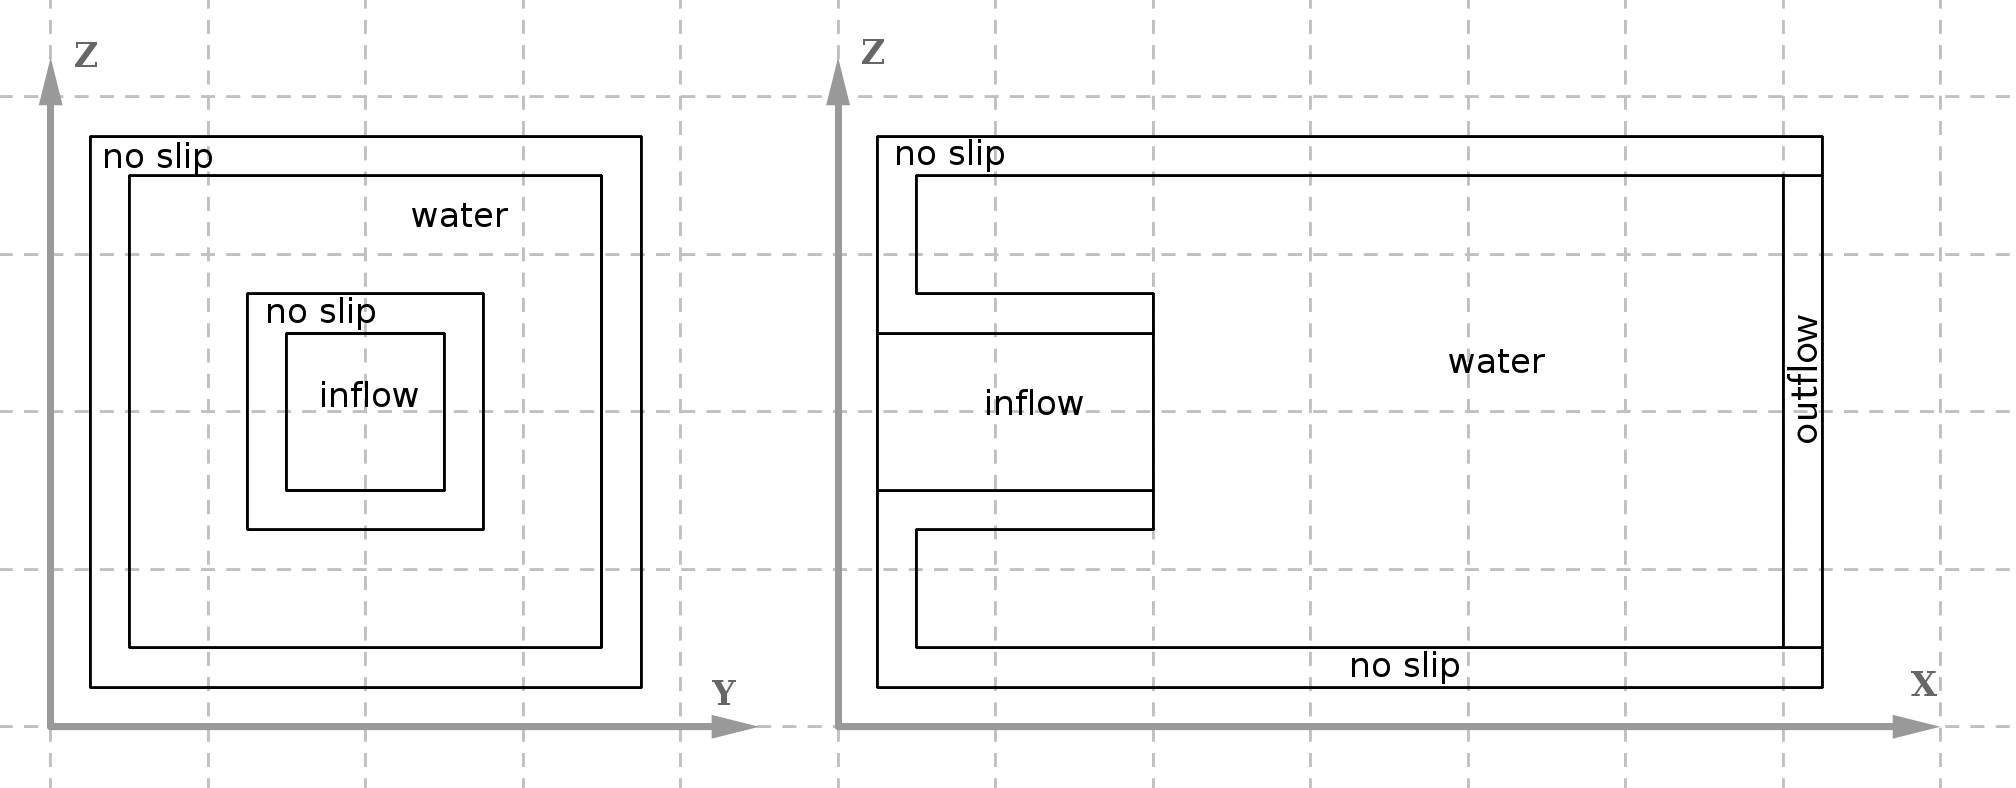
\includegraphics[height=4.1cm]{pipeinflow.png}\\
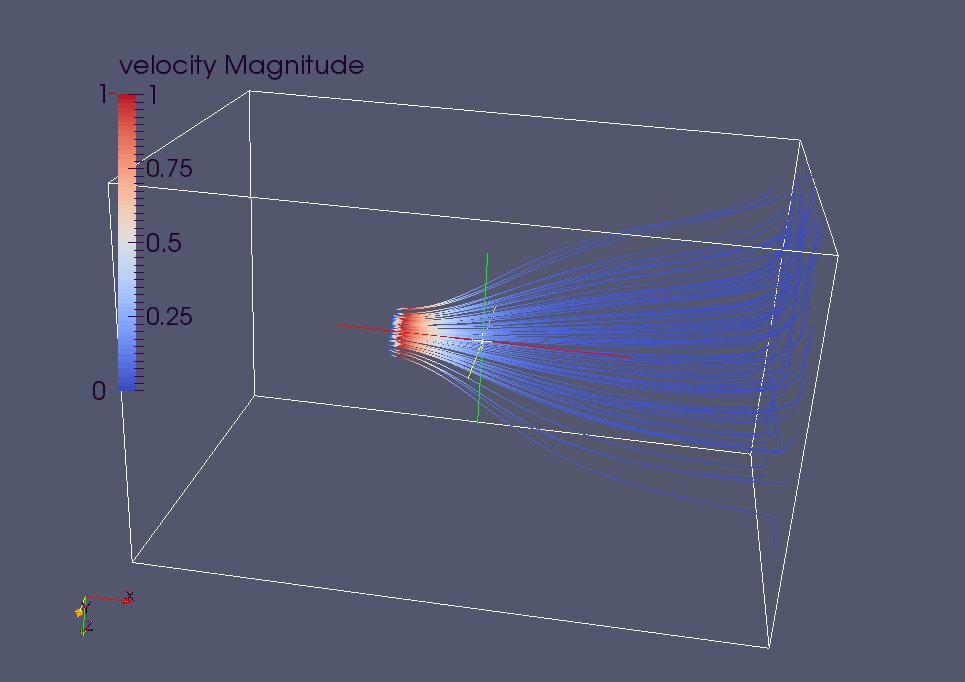
\includegraphics[height=7cm]{pipeinflw.png}
\end{center}

\item Inflow through part of wall, outflow through pipe.
\begin{center}
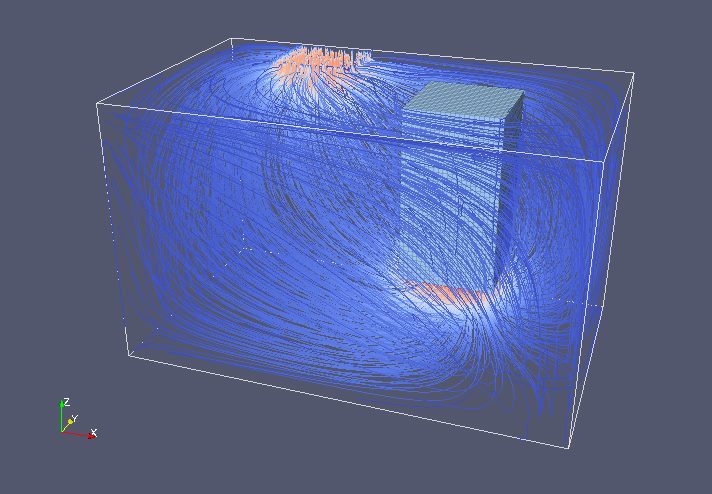
\includegraphics[height=6.5cm]{inoutpipe.jpg}
\end{center}

\newpage
\item Flow over step: streamlines and particle paths.\\
\begin{center}
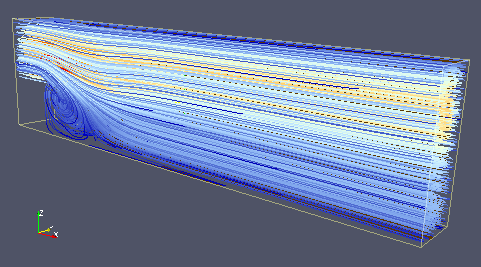
\includegraphics[height=5.4cm]{flowoverstep.png}\\
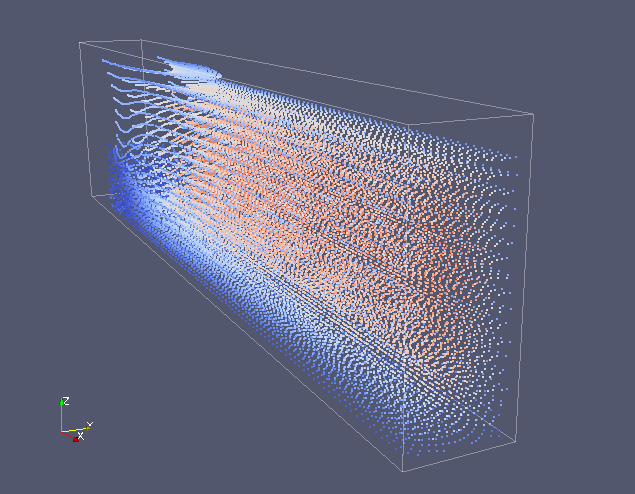
\includegraphics[height=7.7cm]{Step-Particles.png}
\end{center}
\end{itemize}

\begin{thebibliography}{99}
\bibitem{Griebel}
Griebel, M., Dornsheifer, T., Neunhoeffer, T.: \emph{Numerical Simulation in
Fluid Dynamics: A Practical Introduction}. SIAM, {\bf 1998}.

\bibitem{Hirt}
Hirt, C. W., Nichols, B. D.: \emph{Volume of Fluid Method for the Dynamics of Free Boundaries}. Journal of Computational Physics {\bf 39} (1981).

\bibitem{sola}
Hirt, C. W., Nichols, B. D., Hotchkiss, R. S.: \emph{SOLA-VOF: A solution Algorithm for Transient Fluid Flow with Multiple Free Boudaries}. LASL, {\bf 1980}.
\end{thebibliography}

\end{document}
